% Chapter Template

\chapter{Introduction} % Main chapter title

\label{Chapter1} % Change X to a consecutive number; for referencing this chapter elsewhere, use \ref{ChapterX}

\lhead{Chapter 1. \emph{Introduction}} % Change X to a consecutive number; this is for the header on each page - perhaps a shortened title

%----------------------------------------------------------------------------------------
%	SECTION 1
%----------------------------------------------------------------------------------------

%############################# Introduction #################################
\section{Background}
Concrete is the synthetic material currently produced in volumes larger than any other material on Earth. With an annual consumption of approximately 35 billion metric tonnes, it is only second to water in terms of global usage\supercite{mehta2014concrete, Monteiro2017}. It plays a pivotal role in the construction industry, serving as the backbone for buildings, roads, bridges, dams, and many other infrastructure elements central to modern society. Its widespread adoption is the result of its unique combination of properties, including high compressive strength, durability, versatility, and cost-effectiveness\supercite{mehta2014concrete}, rendering it an important asset that directly influences the quality of life and economic development worldwide\supercite{VanDamme2018, Biernacki2017}. Nevertheless, the massive production and use of concrete come with significant environmental challenges. The production of its main constituent, Portland cement, is responsible for 8-9\% of the global anthropogenic CO$_2$ emissions\supercite{Monteiro2017}. Additionally, around 40\% of produced concrete is employed to repair and maintain existing infrastructure\supercite{mehta2014concrete}, which aggravates the environmental impact of concrete. Therefore, the development of more durable and sustainable concrete is of utmost importance, which requires a better understanding of concrete's composition and microstructure. 

Concrete itself is a composite material and can be regarded as a two-phase system\supercite{mehta2014concrete}---the aggregate phase, composed of particles of varying size and shape; and the binding medium, composed of hydrated cement paste. The latter is, in turn, a heterogeneous mixture of different cement hydration products, with calcium silicate hydrate (C-S-H)\footnote{
Conventional cement chemistry notation: C = CaO, S = SiO$_2$, H = H$_2$O
} being the most abundant and important phase. C-S-H makes up 50 to 60\% of the volume of solids in a hydrated cement paste and is responsible for the majority of the long-term strength and durability of concrete\supercite{mehta2014concrete}. Together, the aggregate and binding phases form a complex microstructure that bridges the nanoscale chemistry of hydration products with the properties of concrete at the engineering scale. Nonetheless, the underlying microstructure-property relationships in concrete are not yet fully understood, hindering our ability to manipulate and tailor its properties for specific applications. 


In this context, numerous efforts have been made to understand and model the properties of C-S-H, owing to its central role in determining the properties of concrete\supercite{Ji2012, Papatzani2015, Qomi2020}. Characterisation techniques---such as X-ray diffraction (XRD)\supercite{Allen2007, Houston2009, Oh2012}, nuclear magnetic resonance (NMR)\supercite{Foley2012, Maddalena2019}, and small angle neutron scattering (SANS)---have provided valuable insights into the structure and composition of C-S-H upon which many molecular models have been developed. The pioneering work of Pellenq \emph{et al.}\supercite{Pellenq2009}---which introduced a realistic molecular model of cement hydrates---paved the way for a wide range of molecular modelling techniques\supercite{AbdolhosseiniQomi2014, Richardson2014, Bauchy2014, Kovacevic2016, KunhiMohamed2018} intended to capture the nanoscale structure and properties of C-S-H accurately. Additionally, the advancement of computational power and the development of efficient molecular dynamics (MD) simulation methods have enabled the exploration of mechanical, thermal, and transport properties of C-S-~H\supercite{
AbdolhosseiniQomi2015, Bahraq2022, Cho2020, Barbhuiya2023} under conditions that are relevant to concrete applications but difficult to replicate experimentally. The upscaling of C-S-H properties can be viewed from a hierarchical multiscale perspective, as illustrated in Figure \ref{fig:figure1}, which highlights the microstructure-property relationships of C-S-H at different scales and the relevance of nanoscale properties to the engineering scale of concrete.
\begin{figure}[H]
    \centering
    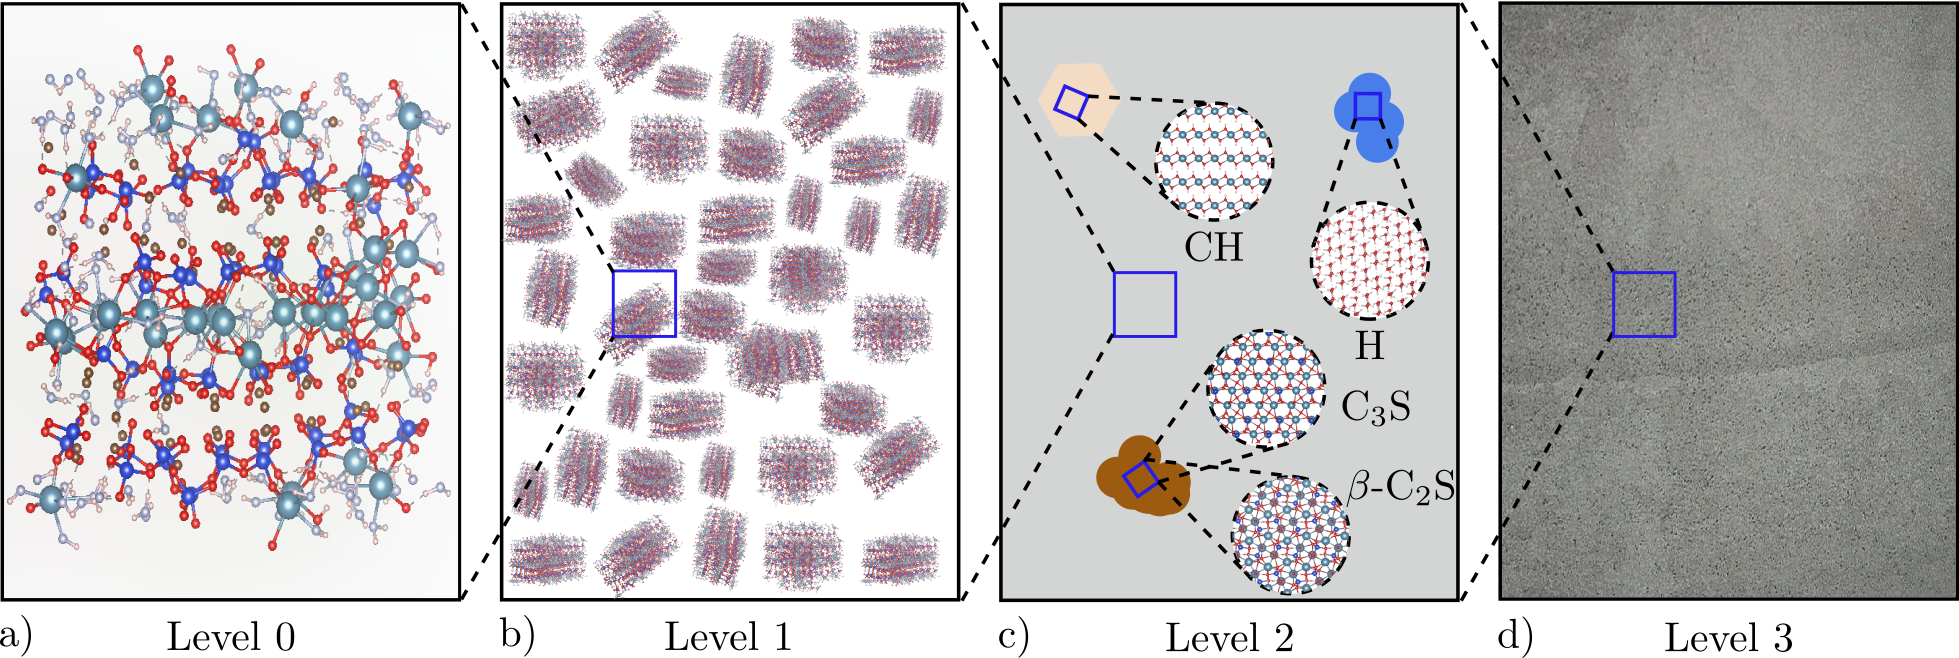
\includegraphics[width=0.9\textwidth]{levels.png}
    \caption{A four-level model representing the upscaling of C-S-H properties from the nanoscale to the engineering scale. (a) snapshot of C-S-H's nanostructure. (b) microstructure of C-S-H created by agglomeration of randomly oriented C-S-H nanoparticles. (c) microtexture of hardened paste composed of hydration products. (d) Macrotexture of cement paste at the engineering scale. Adapted from Ref.\supercite{AbdolhosseiniQomi2015}.}
    \label{fig:figure1}
\end{figure}

Despite the significant progress made in understanding C-S-H at the atomic scale, the inherent complexity of this material makes it challenging to model its structure and properties using classical methods realistically ---primarily molecular dynamics (MD) simulations. Resorting to \emph{ab initio} methods---such as density functional theory (DFT)---can hugely improve the accuracy of these models, but demand high computational resources, making it nearly intractable for real applications\supercite{zotero-item-16}. In this context, machine learning (ML) based concrete research has emerged as a promising approach to address these challenges\supercite{zotero-item-16, Kobayashi2021, Zhu2024}. Trained on large, high-quality \emph{ab initio} datasets, ML models can capture the underlying physics of C-S-H and predict its properties with high accuracy, comparable to that of first-principles methods, while requiring significantly less computational power. 

%-----------------------------------
%	SUBSECTION 1
%-----------------------------------
\section{Problem Statement}
Concrete production is projected to increase by 50\% annually by 2050\supercite{Monteiro2017}, and with no foreseeable alternatives to Portland cement, the urgent need for more sustainable concrete is evident. The development of advanced concrete with enhanced durability and performance could significantly lower the environmental burden. State-of-the-art methods such as machine learning show great potential to accelerate this transition, providing a powerful tool to advance our understanding of concrete's microstructure and properties. 

In this context, this report aims to investigate the performance of a machine learning force field (MLFF) in modelling and predicting the mechanical properties of C-S-H. Such MLFF will be trained and validated
using \emph{ab initio} data, ensuring it captures the complex atomic interactions and structural variability of C-S-H. Ultimately, our goal is to develop a reliable and computationally efficient model that can predict the mechanical properties of C-S-H, thereby supporting concrete research towards a sustainable future.
%-----------------------------------
%	SUBSECTION 2
%-----------------------------------

\section{General and Specific Objectives}
The main goal of this work is to use density functional theory (DFT), \emph{ab initio} molecular dynamics (AIMD), and machine learning (ML) to
develop a machine learning force field (MLFF) for calcium silicate hydrates (C-S-H) to study the mechanical properties of C-S-H. To achieve this, the following specific objectives are defined:
\begin{itemize}
    \item To describe the theoretical foundations of DFT, AIMD, and MLFFs, including key concepts on exchange-correlation functionals such as PBE and PBEsol, and pseudopotentials. 
    \item To perform geometric relaxation on bulk C-S-H model employing the VASP software with the PBEsol functional.
    \item To analyse the electronic structure of C-S-H by computing the density of states (DOS) of C-S-H.
    \item To train, refit, and test an MLFF using AIMD simulations. 
    \item To compute the equation of state (EOS) and mechanical properties of C-S-H using the MLFF and simulated annealing methods.
    \item To evaluate the transferability of the MLFF by computing the thermal expansion coefficient of C-S-H. 
\end{itemize}
%----------------------------------------------------------------------------------------
%	SECTION 2
%----------------------------------------------------------------------------------------

\section{Overview}
The remainder of this report is organised in the following manner: Chapter \ref{Chapter2} introduces the theoretical framework of the computational methods utilised in this work, including DFT, AIMD, and MLFFs. Chapter \ref{Chapter3} presents the methodology employed to generate the results presented in this report, describing the molecular model of C-S-H, the computational setup, and the MLFF generation process. Then, Chapter \ref{Chapter4} presents the results of our computational investigations. Ultimately, Chapter \ref{Chapter5} finalises this report, the main conclusions about the work done are drawn, and the outlook for future work is discussed.
